\begin{center}
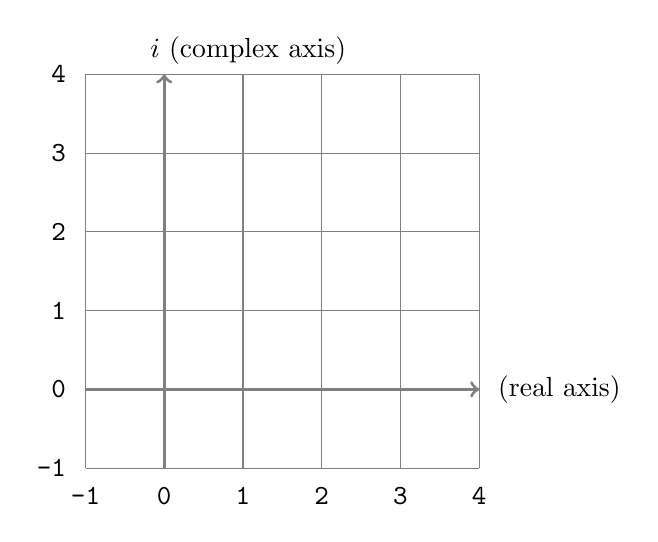
\begin{tikzpicture}
\draw[gray] (-1,-1) to  (-1,4);
\draw[gray] (0,-1) to  (0,4);
\draw[gray] (1,-1) to  (1,4);
\draw[gray] (2,-1) to  (2,4);
\draw[gray] (3,-1) to  (3,4);
\draw[gray] (4,-1) to  (4,4);
\draw[gray] (-1,-1) to  (4,-1);
\draw[gray] (-1,0) to  (4,0);
\draw[gray] (-1,1) to  (4,1);
\draw[gray] (-1,2) to  (4,2);
\draw[gray] (-1,3) to  (4,3);
\draw[gray] (-1,4) to  (4,4);
\draw(-1, -1) node [font=\ttfamily, label=below:{\normalsize {\texttt{-1}}}] {};
\draw(0, -1) node [font=\ttfamily, label=below:{\normalsize {\texttt{0}}}] {};
\draw(1, -1) node [font=\ttfamily, label=below:{\normalsize {\texttt{1}}}] {};
\draw(2, -1) node [font=\ttfamily, label=below:{\normalsize {\texttt{2}}}] {};
\draw(3, -1) node [font=\ttfamily, label=below:{\normalsize {\texttt{3}}}] {};
\draw(4, -1) node [font=\ttfamily, label=below:{\normalsize {\texttt{4}}}] {};
\draw(-1, -1) node [font=\ttfamily, label=left:{\normalsize {\texttt{-1}}}] {};
\draw(-1, 0) node [font=\ttfamily, label=left:{\normalsize {\texttt{0}}}] {};
\draw(-1, 1) node [font=\ttfamily, label=left:{\normalsize {\texttt{1}}}] {};
\draw(-1, 2) node [font=\ttfamily, label=left:{\normalsize {\texttt{2}}}] {};
\draw(-1, 3) node [font=\ttfamily, label=left:{\normalsize {\texttt{3}}}] {};
\draw(-1, 4) node [font=\ttfamily, label=left:{\normalsize {\texttt{4}}}] {};
\draw[line width=0.04cm,black!50,->] (-1,0) to  (4,0);
\draw[line width=0.04cm,black!50,->] (0,-1) to  (0,4);

\node[anchor=west] at (4,0)   {$\R$ (real axis)};

\node[anchor=west] at (-0.3,4.3)   {$i\R$ (complex axis)};
\end{tikzpicture}

\end{center}

